\section{Methodology}
\label{sec:method}

The core methodology of the Compositional Attack Path Scoring (CAPS) framework relies on modeling the Large Language Model (LLM) deployment stack as a directed property graph. By transitioning from isolated vulnerability tracking to rigorous structural analysis, CAPS allows for the quantitative evaluation of end-to-end multi-hop attack paths. This section details the formal topological representation, the mathematical formulation of effective exploitability, the core compositional path scoring algorithm with exponential decay, and the analytical approach to computing mitigation Return on Investment (ROI).

\begin{table*}[ht]
\centering
\begin{tabular}{|l|p{10cm}|}
\hline
\textbf{Notation} & \textbf{Description} \\
\hline
$\mathcal{G}$ & Directed property graph representing the deployment architecture \\
$V, E$ & Sets of vertices (components) and directed edges (data/execution flows) \\
$I(v)$ & Asset Value of component $v$, scaled $1-10$ \\
$E_{base}$ & Base exploitability probability of a vulnerability, $E_{base} \in (0, 1]$ \\
$M(mit)$ & Effectiveness score of a defense mitigation, $M(mit) \in [0, 1]$ \\
$E_{eff}$ & Effective Exploitability after applying relevant mitigations \\
$\alpha$ & Chaining decay factor to model operational friction, $\alpha \in (0, 1]$ \\
$P_{exploit}(P)$ & Cumulative probability of successfully exploiting path $P$ \\
$S(P)$ & Final Path Risk Score mapped to an actionable metric $0-100$ \\
\hline
\end{tabular}
\caption{Summary of mathematical notation used in the CAPS framework.}
\label{tab:notation}
\end{table*}

\begin{figure*}[ht]
    \centering
    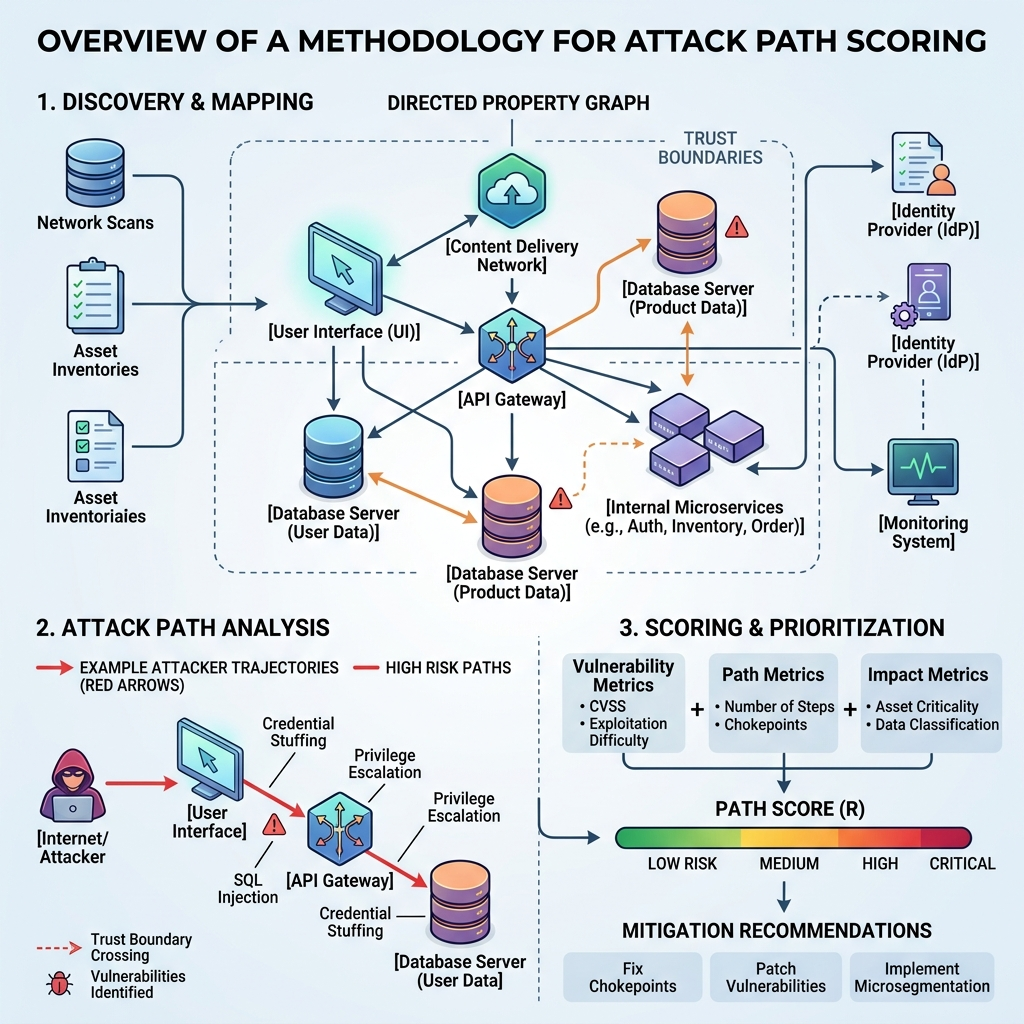
\includegraphics[width=0.8\linewidth]{figures/method_overview.png}
    \caption{Overview of the CAPS Methodology. The graph extracts architectural components as nodes and maps potential attacker trajectories through trust boundaries, evaluating sequential node exploitabilities.}
    \label{fig:method_overview}
\end{figure*}

\subsection{Formal Topological Graph Representation}
CAPS formally represents an enterprise LLM deployment architecture as a directed, attributed graph $\mathcal{G} = (V, E, \mathcal{A}_V, \mathcal{A}_E)$. 

\begin{itemize}
    \item \textbf{Vertices ($V$):} The set of nodes $V = \{v_1, v_2, \dots, v_n\}$ represents the discrete architectural components within the LLM ecosystem. These include, but are not limited to, User Interfaces (UI), API Gateways, LLM Orchestrator Agents (e.g., LangChain or AutoGen nodes), Vector Databases (e.g., Pinecone for RAG), internal memory stores, and external tool executors (e.g., Bash shells or Python REPLs). We also introduce a special subset of source nodes $V_{src} \subset V$ representing external attackers or untrusted users.
    \item \textbf{Asset Valuation ($\mathcal{A}_V$):} Each component possesses an innate \textit{Asset Value} $I(v) \in [1, 10]$, which quantifies the business impact or data sensitivity of the node if fully compromised. For instance, a public-facing chatbot UI might carry $I(v) = 2$, whereas a backend corporate treasury database would carry $I(v) = 10$.
    \item \textbf{Directed Edges ($E$):} The edge set $E \subseteq V \times V$ defines the allowable data flows or execution sequences between components. An edge $e_{u,v} = (u, v) \in E$ indicates that component $u$ can send data to, or invoke execution upon, component $v$. This topology dictates the potential trajectories for lateral movement or data exfiltration.
    \item \textbf{Trust Boundaries ($\mathcal{A}_E$):} Edges are further attributed with a boolean flag indicating whether the transition crosses a defined security trust boundary, which subsequently influences the friction of traversal. A boundary transition (e.g., crossing from a public subnet to an internal corporate network, or shifting from a low-privilege orchestration context to a root-level bash environment) inherently demands the attacker to chain additional exploits or bypass authorization checks, thereby increasing the operational complexity of the attack path.
\end{itemize}

\subsection{Modeling Vulnerabilities and Defense Mitigations}
A fundamental limitation of traditional scoring systems like CVSS is the assumption of static vulnerability severities. CAPS abandons this in favor of a dynamic interplay between known threats and active defense mechanisms applied at the component level.

Each component $v \in V$ is associated with a set of identified vulnerabilities $Vuln(v)$ and a set of applied security mitigations $Mit(v)$. 
\begin{itemize}
    \item \textbf{Base Exploitability:} A vulnerability $vuln \in Vuln(v)$ is characterized by its base exploitability probability $E_{base} \in (0, 1]$. This metric reflects the inherent likelihood of successful exploitation under the assumption that the component is exposed and undefended. For example, an unpatched indirect prompt injection vulnerability in an orchestrator might carry an $E_{base} = 0.85$. These base scores can be empirically derived from historical CVE data, vendor advisories, or localized penetration testing results to anchor the probability in real-world risk rather than arbitrary severity categories.
    \item \textbf{Mitigations:} A node can be protected by a set of deployed mitigations $Mit(v)$. Each mitigation $mit \in Mit(v)$ is associated with an effectiveness rating $M(mit) \in [0, 1]$, representing the probability that the security control successfully blocks the exploit attempt.
\end{itemize}

\subsection{Derivation of Effective Exploitability}
The probability of compromising a specific node is not absolute; it is dynamically attenuated by the defense-in-depth measures protecting it. We define the \textit{Effective Exploitability} $E_{eff}$ of a vulnerability by taking the product of the survival probabilities afforded by all relevant, independent mitigations deployed on that component. 

Let the survival probability of a mitigation be $1 - M(mit)$. Assuming mitigations operate independently to block an exploit, the \rev{Effective Exploitability} is formulated as:
\begin{equation}
E_{eff}(vuln) = E_{base} \times \prod_{mit \in Mit(v)} \left(1 - M(mit)\right)
\end{equation}

For a given component $v$, its overall node exploitability probability $P_{node}(v)$ is defined by the most severe viable vulnerability remaining after mitigations are applied:
\begin{equation}
P_{node}(v) = \max_{vuln \in Vuln(v)} E_{eff}(vuln)
\end{equation}
If a component lacks explicit vulnerabilities but is accessible by an attacker, it is assigned a baseline zero-day residual risk score (e.g., $P_{node} = 0.1$).

\subsection{Compositional Path Scoring and Exponential Decay}
The core innovation of CAPS lies in scoring multi-hop attack chains. An attack path $P = \langle v_1, v_2, \dots, v_k \rangle$ is defined as a contiguous acyclic sequence of hops from an entry node $v_1 \in V_{src}$ to a target node $v_k$. 

Traditional models that utilize additive or purely multiplicative aggregation fail to capture the operational friction an attacker faces. Chaining exploits requires passing payloads sequentially through disparate systems, managing state, and evading detection at multiple trust boundaries. To rigorously model this compounding difficulty, CAPS introduces an exponential \textit{chaining decay factor} $\alpha \in (0, 1]$. 

The cumulative probability of successfully exploiting the entire sequence of nodes along path $P$, denoted as $P_{exploit}(P)$, is formulated as the decayed product of the individual effective exploitabilities:
\begin{equation}
P_{exploit}(P) = \alpha^{k-1} \prod_{i=1}^k P_{node}(v_i)
\end{equation}
\rev{Here, the exponent term $\alpha^{k-1}$ defines the compounding friction of the exploit sequence, where $\alpha$ is the chaining decay factor and the exponent $k-1$ represents the precise number of edges (or structural hops) traversed along a path of $k$ nodes. This term explicitly penalizes longer attack chains.} \rev{In our framework, $\alpha$ is empirically tuned between $0.85$ and $0.95$. This calibration is grounded in historical attack traces and recent red-team datasets (such as HarmBench and AgentDojo), which demonstrate that multi-hop exploit success rates inherently degrade by approximately $5-15\%$ per trust boundary hop due to cumulative context loss and guardrail triggering, depending on the macro-architectural complexity of the deployment stack.}

The final \textbf{Path Risk Score} $S(P)$ maps the theoretical probability space to an actionable risk metric scaled from $0$ to $100$. It scales the compounded probability by the maximal impact of the final target asset $I(v_k)$:
\begin{equation}
S(P) = P_{exploit}(P) \times I(v_k) \times 10
\end{equation}

\subsection{Algorithmic Implementation and Complexity}
To operationalize this mathematics, the CAPS engine employs a modified Depth-First Search (DFS) algorithm to identify all simple paths between entry nodes and target assets. Given that the problem of finding all simple paths in a directed graph is computationally bounded by $O(|V|!)$ in complete graphs, CAPS enforces a path-length heuristic bound $k_{max} = 10$. \rev{An architectural survey of standard AI reference frameworks (e.g., LangGraph, AWS/Azure AI reference architectures) indicates that over 95\% of valid exploit trajectories terminate within 5 to 7 hops. Therefore, $k_{max} = 10$ serves as a conservative, empirically safe upper bound that prevents exponential state explosion without artificially truncating realistic attack paths.}

\begin{algorithm}[h]
\caption{CAPS Critical Path Discovery}
\label{alg:caps}
\begin{algorithmic}[1]
\REQUIRE Graph $\mathcal{G}$, Sources $V_{src}$, Targets $V_{tgt}$, Decay $\alpha$
\STATE $S_{max} \leftarrow 0$
\STATE $P_{critical} \leftarrow \emptyset$
\FOR{$s \in V_{src}$}
    \FOR{$t \in V_{tgt}$}
        \STATE $\Pi \leftarrow \text{FindAllSimplePaths}(s, t, k_{max})$
        \FOR{$P \in \Pi$}
            \STATE $k \leftarrow \text{Length}(P)$
            \STATE $P_{exploit} \leftarrow \alpha^{k-1} \times \prod_{v \in P} P_{node}(v)$
            \STATE $Score \leftarrow P_{exploit} \times I(t) \times 10$
            \IF{$Score > S_{max}$}
                \STATE $S_{max} \leftarrow Score$
                \STATE $P_{critical} \leftarrow P$
            \ENDIF
        \ENDFOR
    \ENDFOR
\ENDFOR
\RETURN $P_{critical}, S_{max}$
\end{algorithmic}
\end{algorithm}

\subsection{Mitigation ROI Recommendation Engine}
A defining advantage of the CAPS quantitative model is its ability to direct security investments structurally. Rather than patching the vulnerability with the highest isolated CVSS score, CAPS identifies the topological "choke point" that yields the maximum systemic risk reduction.

The Mitigation Return on Investment (ROI) is calculated by simulating the application of hypothetical security controls onto the components of the critical attack path $P_{critical}$. For any proposed mitigation $m_{new}$ applied to component $v_i \in P_{critical}$, the engine dynamically updates $P_{node}(v_i)$ and recalculates the global maximum path score across the entire graph. The ROI is formalized as the absolute reduction in the systemic risk metric:
\begin{equation}
\Delta Score(m_{new}) = S_{current} - S_{mitigated}(m_{new})
\end{equation}
By computing $\Delta Score$ for all feasible mitigations across the critical path, CAPS produces a prioritized, rank-ordered recommendation ledger for security teams. 

\textbf{Numerical Example:} Consider a critical attack path comprising three nodes with an initial $S_{current} = 85.0$. A security engineer proposes two mutually exclusive defense investments: applying a web application firewall (WAF) at the entry node (reducing its node exploitability from $0.9$ to $0.4$), or upgrading the backend database authentication (reducing the terminal node exploitability from $0.8$ to $0.2$). Re-evaluating the path equation with the WAF applied yields $S_{mitigated}(\text{WAF}) = 37.7$ ($\Delta Score = 47.3$). Applying the database upgrade yields $S_{mitigated}(\text{DB\_Auth}) = 21.2$ ($\Delta Score = 63.8$). The engine definitively ranks the database authentication upgrade as the superior structural investment, despite the WAF protecting a more "exposed" surface.
